%!TeX encoding = UTF-8
%!BIB program = biber

\documentclass[12pt,a4paper,UTF8]{ctexart}

% ==============================
% 基础宏包
% ==============================
\usepackage[top=2.5cm,bottom=2.5cm,left=2cm,right=2cm,bindingoffset=0.5cm]{geometry}
\usepackage{fancyhdr}
\usepackage{titlesec}
\usepackage{graphicx}
\usepackage{enumitem}
\usepackage{indentfirst}
\usepackage{amsmath}
\usepackage{url}
\usepackage{booktabs}
\usepackage{array}
\usepackage[hidelinks]{hyperref}
\usepackage[backend=biber, style=gb7714-2015]{biblatex}

\addbibresource{ref.bib}

% ==============================
% 加载排版组件
% ==============================
% ==============================
% 标题命令
% ==============================
\newcommand{\makereporttitle}{%
  \begin{center}
    \vspace{0.5cm}
    {\heiti\erhao \mucdoctitle\par}
    \vspace{0.8cm}
  \end{center}
}

% ==============================
% 学生信息命令（水平排列）
% ==============================
\newcommand{\makestudentinfo}{%
  \begin{center}
    {\songti\xiaosi
    姓名：\underline{\makebox[3cm][c]{\varmucauthor}}%
    \hspace{2em}%
    学号：\underline{\makebox[3cm][c]{\varmucstudentid}}%
    \hspace{2em}%
    班级：\underline{\makebox[3cm][c]{\varmucclass}}%
    \par}
  \end{center}
  \vspace{0.3cm}
}

% ==============================
% 以下为兼容旧版封面命令（URTP 论文封面）
% ==============================
\newcommand{\fontstxs}{\fontsize{15pt}{17pt} \selectfont \songti{}}
\newcommand{\fontstsh}{\fontsize{14pt}{16pt} \selectfont \songti{}}
\newcommand{\fonthtxe}{\fontsize{18pt}{20pt} \selectfont \heiti{}}

\newcommand{\makecover}{%
  \thispagestyle{empty}
  \begin{center}
    \vspace*{1cm}
    \noindent

    \begin{minipage}[c]{2.17cm}
      
\includegraphics[width=\linewidth]{assets/MUC.jpg}
    \end{minipage}
    \hspace{0.5cm}
    \begin{minipage}[c]{0.8\textwidth}
      {\fontsize{18pt}{20pt}\selectfont \heiti{}
      中央民族大学大学生创新训练计划结题论文\\[0.3cm]}
      {\fontsize{12pt}{14pt}\fontfamily{phv} \selectfont \bfseries
      URTP Final Thesis of Minzu University of China}
    \end{minipage}

    \vspace{4cm}
    \makedoctitle{}
    \vspace{0.5cm}
    \makedocsubtitle{}
    \vspace{6cm}

    \begin{tabular}{ll}
      {\fontstxs{} 计划编号：} & \underline{\fontstxs{} \makebox[6cm][c]{\varmucprojectid}}\\
      {\fontstxs{} 项目类型：} & \underline{\fontstxs{} \makebox[6cm][c]{\varmucprojecttype}}\\
      {\fontstxs{} 指导教师：} & \underline{\fontstxs{} \makebox[6cm][c]{\varmucprojectteacher}}\\
      {\fontstxs{} 项目成员：} & \underline{\fontstxs{} \makebox[6cm][c]{\varmucprojectmembers}}\\
      {\fontstxs{} 依托单位：} & \underline{\fontstxs{} \makebox[6cm][c]{\varmucprojectunit}}\\
    \end{tabular}

    \vspace{3cm}

    {\fontstsh{} \varmucprojectdate{}}
  \end{center}
  \clearpage
}
\newcommand{\setupHeader}{
    \renewcommand{\baselinestretch}{1.25}
    \setlength{\parindent}{2em}

    % 页眉页脚
    \pagestyle{fancy}
    \setlength{\headheight}{14.5pt}
    \setlength{\headsep}{15pt}
    \fancyhf{}
    \fancyhead[C]{\songti\zihao{5}中央民族大学课程实验报告}
    \renewcommand{\headrulewidth}{0.5pt}
    \fancyfoot[C]{\songti\zihao{5}\thepage}
}
\makeatletter
\def\mucdoctitle{}
\makeatother

\newcommand{\doctitle}[1]{%
  \def\mucdoctitle{#1}%  不需要 \makeatletter，因为没用到 @
}

\newcommand{\makedoctitle}{%
  \songti\zihao{3}%
  \mucdoctitle
}

\makeatletter
\def\mucdocsubtitle{}
\makeatother

\newcommand{\docsubtitle}[1]{%
  \makeatletter
  \def\mucdocsubtitle
{#1}%
  \makeatother
}

\newcommand{\makedocsubtitle}{%
  \makeatletter
  {\fontsize{16pt}{18pt} \selectfont \heiti{}%
\ifx\mucdocsubtitle\empty\else ——\mucdocsubtitle\fi}
  \makeatother
}

\makeatletter
\def\varmucprojectid{}
\makeatother

\newcommand{\mucprojectid}[1]{%
  \makeatletter
  \def\varmucprojectid{#1}%
  \makeatother
}

\makeatletter
\def\varmucprojecttype{}
\makeatother

\newcommand{\mucprojecttype}[1]{%
  \makeatletter
  \def\varmucprojecttype{#1}%
  \makeatother
}

\makeatletter
\def\varmucprojectteacher{}
\makeatother

\newcommand{\mucprojectteacher}[1]{%
  \makeatletter
  \def\varmucprojectteacher{#1}%
  \makeatother
}

\makeatletter
\def\varmucauthor{}
\makeatother

\newcommand{\mucauthor}[1]{%
  \makeatletter
  \def\varmucauthor{#1}%
  \makeatother
}

\makeatletter
\def\varmucstudentid{}
\makeatother

\newcommand{\mucstudentid}[1]{%
  \makeatletter
  \def\varmucstudentid{#1}%
  \makeatother
}

\makeatletter
\def\varmucclass{}
\makeatother

\newcommand{\mucclass}[1]{%
  \makeatletter
  \def\varmucclass{#1}%
  \makeatother
}

\newcommand{\makeauthorinfo}{%
  {%
    \begin{center}
      \par\noindent
      \songti\fontsize{16pt}{20pt}\selectfont
      \varmucauthor{}，\varmucclass{}，\varmucstudentid{}%
    \end{center}
  }%
}

% ==============================
% URTP 封面用变量
% ==============================
\makeatletter
\def\varmucprojectmembers{}
\def\varmucprojectunit{}
\def\varmucprojectdate{}
\makeatother

\newcommand{\mucprojectmembers}[1]{%
  \makeatletter
  \def\varmucprojectmembers{#1}%
  \makeatother
}

\newcommand{\mucprojectunit}[1]{%
  \makeatletter
  \def\varmucprojectunit{#1}%
  \makeatother
}

\newcommand{\mucprojectdate}[1]{%
  \makeatletter
  \def\varmucprojectdate{#1}%
  \makeatother
}
\makeatletter
\def\muckeywords{} % @符号变量需包裹
\def\mucenglishkeywords{} % @符号变量需包裹
\makeatother

\newcommand{\keywords}[1]{%
  \makeatletter
  \def\muckeywords{#1}%
  \makeatother
}

% 关键字生成
\newcommand{\makekeywords}{%
  \makeatletter
  \par\noindent
  {\songti\xiaosi\textbf{关键字：}}%
  {\songti\xiaosi\space \muckeywords}%
  \makeatother
  \vspace{0.5cm}
}

\newsavebox{\abstractbox}
\newenvironment{MUCAbstract}{%
  \begin{lrbox}{\abstractbox}
    \minipage{\linewidth}  % 保证盒子宽度正常
    \songti\xiaosi
}{%
    \endminipage
  \end{lrbox}
  \phantomsection
  \addcontentsline{toc}{section}{摘要}%
  \par\noindent
  \songti\xiaosi
  \textbf{摘要：}\usebox{\abstractbox}%
  \par
  \vspace{0.5cm}
}

\setupHeader{}

% ==============================
% 字号定义
% ==============================
\newcommand{\erhao}{\fontsize{22pt}{\baselineskip}\selectfont}  % 二号 22pt
\newcommand{\sanhao}{\fontsize{16pt}{\baselineskip}\selectfont}  % 三号 16pt
\newcommand{\sihao}{\fontsize{14pt}{\baselineskip}\selectfont}   % 四号 14pt
\newcommand{\xiaosi}{\fontsize{12pt}{\baselineskip}\selectfont}  % 小四 12pt

% ==============================
% 节标题格式
% ==============================
% section: 黑体加粗三号, "1." 编号
\titleformat{\section}{\bfseries\heiti\sanhao}{\thesection.}{1em}{}
\titlespacing*{\section}{0pt}{18pt}{12pt}
% subsection: 宋体加粗四号, "(1)" 编号
\renewcommand{\thesubsection}{\arabic{subsection}}
\titleformat{\subsection}{\bfseries\songti\sihao}{(\thesubsection)}{1em}{}
\titlespacing*{\subsection}{0pt}{12pt}{6pt}
% subsubsection: 宋体小四, "▸" 前缀
\titleformat{\subsubsection}{\songti\xiaosi}{$\triangleright$\enspace}{0pt}{}
\titlespacing*{\subsubsection}{0pt}{8pt}{4pt}

% ==============================
% 列表格式
% ==============================
\setlist[enumerate,1]{label=(\arabic*),leftmargin=2em}
\setlist[enumerate,2]{label=\alph*.,leftmargin=4em}

% ==============================
% 加载用户数据
% ==============================
\doctitle{《材科基实验-热重》实验报告}
\docsubtitle{}
\keywords{热重分析；材料科学基础；实验报告}
\mucauthor{刘佳鹏}
\mucstudentid{24012639}
\mucclass{纳米二班}
% URTP 封面信息（可选）
% \mucprojectid{计划编号}
% \mucprojecttype{项目类型}
% \mucprojectteacher{指导教师}
% \mucprojectmembers{项目成员}
% \mucprojectunit{依托单位}
% \mucprojectdate{日期}

\begin{document}

% ---------- 校徽（右上角） ----------
{
  \raggedleft
  
\includegraphics[width=2.5cm]{assets/MUC.jpg}
  \par
}

% ---------- 标题 ----------
\makereporttitle{}

% ---------- 学生信息 ----------
\makestudentinfo{}

% ---------- 关键字 ----------
\makekeywords{}

% ---------- 摘要 ----------
\begin{MUCAbstract}
    本实验采用热重分析法（TGA）对五水合硫酸铜（$\mathrm{CuSO_4 \cdot 5H_2O}$）进行热分解测试，
    通过分析TG曲线和DSC曲线，研究其分步失水过程。
    实验结果表明硫酸铜的脱水过程呈现明显的阶段性特征，
    各阶段对应不同结合状态结晶水的逐步脱除。
\end{MUCAbstract}

% ---------- 正文（单栏） ----------
% ==============================
% 正文区
% ==============================

\section{引\hspace{1em}言}

热重分析（Thermogravimetric Analysis, TGA）是在程序控制温度下，测量物质的质量与温度或时间关系的一种热分析技术。它广泛应用于材料热稳定性评价、组成分析、热分解动力学研究等领域。通过TGA曲线，可以获得材料的热分解温度、失重率、热分解活化能等重要参数，为材料的选择、加工和应用提供重要的理论依据。

本实验旨在通过热重分析法对五水合硫酸铜（$\mathrm{CuSO_4 \cdot 5H_2O}$）进行热分解测试，掌握热重分析的基本原理和操作方法，学会分析TG（热重）曲线和DSC（差示扫描量热）曲线，通过TG-DSC曲线分析硫酸铜的分步失水过程。

\section{实验原理与方法}

\subsection{热重分析法}

\subsubsection{实验原理}

热重分析的基本原理是：在程序控温条件下，利用热天平连续测量样品质量随温度（或时间）的变化。当样品在加热过程中发生升华、汽化、分解出气体或失去结晶水等物理化学变化时，其质量会相应发生变化。通过记录样品质量与温度的关系，即可得到热重曲线（TG曲线）。

对TG曲线进行一阶微分处理，可获得微分热重曲线（DTG曲线）。DTG曲线反映的是质量变化速率随温度的变化关系，其峰顶温度对应最大失重速率温度（$T_p$）。DTG曲线能够更清晰地显示样品在各温度区间的失重行为，有助于分析重叠的热分解过程。

TG-DTG曲线的典型特征参数包括：
\begin{itemize}
    \item 起始分解温度（$T_i$）：样品开始明显失重的温度；
    \item 外推起始温度（$T_{onset}$）：由TG曲线最大斜率处切线与基线延长线的交点确定；
    \item 最大失重速率温度（$T_p$）：DTG曲线的峰顶温度；
    \item 终止温度（$T_f$）：失重过程基本结束的温度；
    \item 总失重率（$\Delta m$）：样品在整个升温过程中的质量损失百分比。
\end{itemize}

\subsubsection{实验流程}

热重分析实验的主要流程如下：

\begin{enumerate}[label=(\arabic*)]
    \item \textbf{样品制备}：取适量待测样品（通常5--15 mg），研磨均匀后置于坩埚中。样品用量不宜过多，以免传热不均导致测试误差；
    \item \textbf{仪器校准}：使用标准砝码对热天平进行质量校准，使用标准物质（如居里点标准磁性材料）进行温度校准；
    \item \textbf{参数设置}：设定升温程序（包括起始温度、终止温度、升温速率等），选择实验气氛（氮气、空气、氩气等）及气体流量；
    \item \textbf{基线校正}：在相同实验条件下进行空白实验，获得基线，用于扣除浮力效应和气体对流等系统误差；
    \item \textbf{正式测试}：将装样坩埚放入热天平中，启动升温程序，实时记录样品质量随温度的变化；
    \item \textbf{数据分析}：导出TG和DTG曲线数据，确定特征温度，分析失重过程，计算热分解动力学参数。
\end{enumerate}

\subsubsection{注意事项}

\begin{enumerate}[label=(\arabic*)]
    \item \textbf{样品用量}：样品量一般控制在5--15 mg，过多会导致温度梯度增大，影响测试精度；过少则信噪比低，数据波动大；
    \item \textbf{升温速率}：常用升温速率为5、10、20 $\mathrm{^\circ C/min}$。升温速率越快，TG曲线向高温方向偏移，特征温度偏高；升温速率越慢，分辨率越高，但实验耗时增长；
    \item \textbf{气氛选择}：惰性气氛（如$\mathrm{N_2}$、Ar）用于研究热分解行为；氧化性气氛（如空气、$\mathrm{O_2}$）用于研究氧化稳定性。气体流量通常控制在20--100 mL/min；
    \item \textbf{坩埚选择}：根据样品性质和测试温度范围选择合适的坩埚材质（$\mathrm{Al_2O_3}$、Pt、Al等），使用前应经高温灼烧处理去除杂质；
    \item \textbf{基线漂移}：因浮力效应和气体对流导致的基线漂移应在数据处理时予以扣除；
    \item \textbf{安全操作}：注意高温防护，避免触碰加热炉体，测试完成后待炉体冷却至室温再取出样品。
\end{enumerate}

\section{实验结果与讨论}

\subsection{TG-DSC曲线分析}

图\ref{fig:tg-dtg}为五水合硫酸铜（$\mathrm{CuSO_4 \cdot 5H_2O}$）在空气气氛下测得的TG-DSC曲线。从图中可以清晰地观察到，硫酸铜的脱水过程呈现明显的多阶段特征，TG曲线呈阶梯状下降，DSC曲线在对应温度区间出现若干吸热峰。

\begin{figure}[htbp]
    \centering
    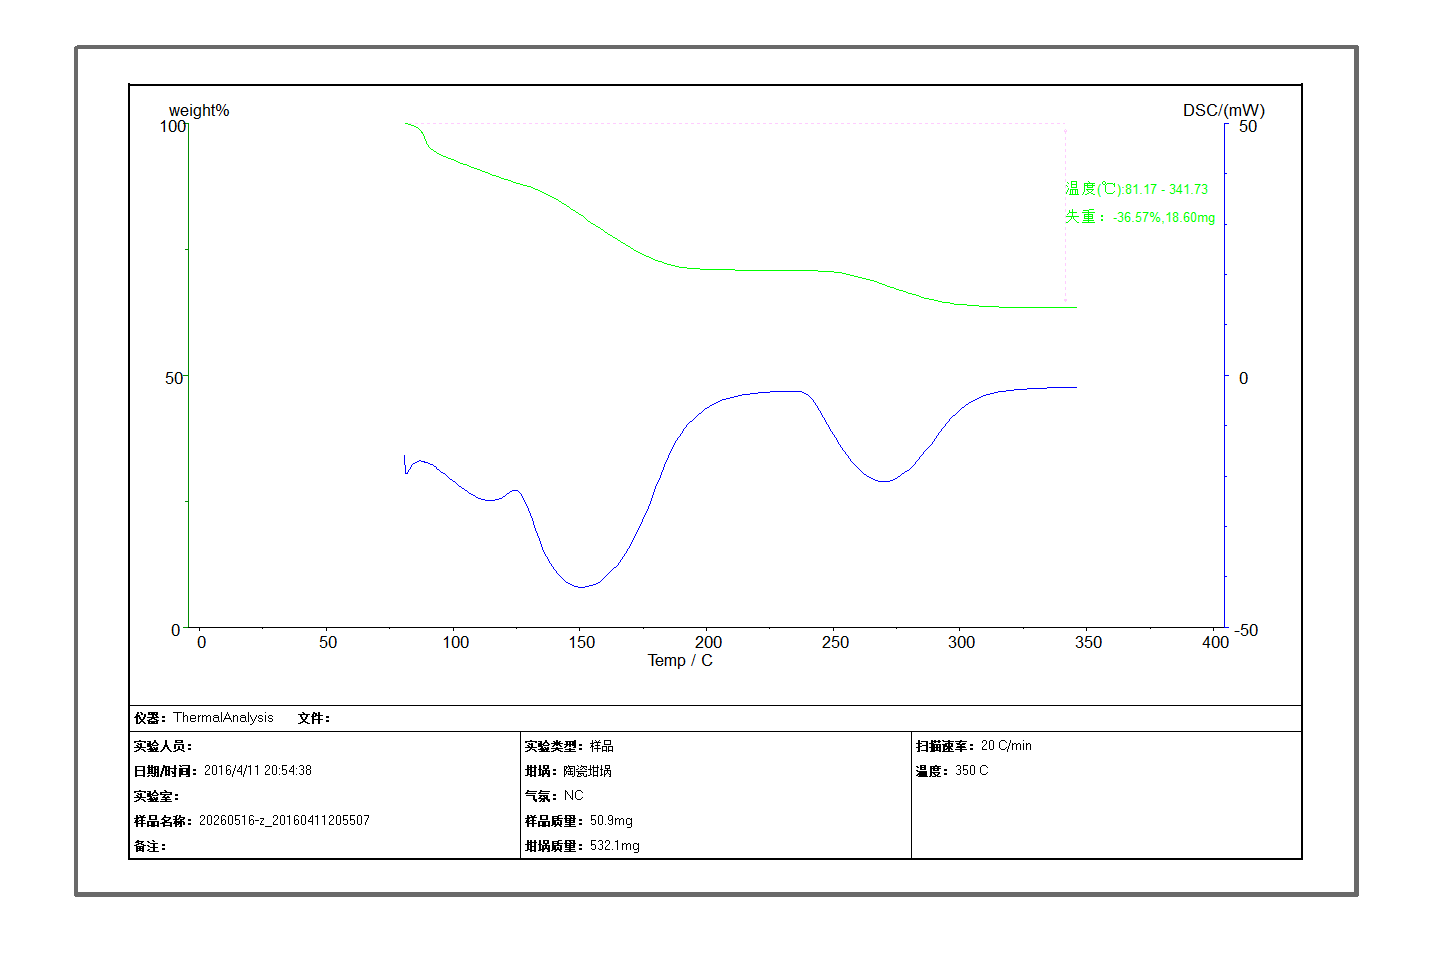
\includegraphics[width=\textwidth]{data/tg_dtg_curve.png}
    \caption{$\mathrm{CuSO_4 \cdot 5H_2O}$在空气气氛下的TG-DSC曲线}
    \label{fig:tg-dtg}
\end{figure}

根据TG-DSC曲线的变化特征，可将硫酸铜的脱水过程大致划分为以下两个阶段：

\begin{enumerate}[label=(\arabic*)]
    \item \textbf{第一阶段（低温区，约80--130\,$\mathrm{^\circ C}$）}：该阶段TG曲线出现明显失重，DSC曲线对应出现一个尖锐的吸热峰。此阶段对应于五水合硫酸铜中部分结晶水的脱除。由于这部分结晶水与铜离子的结合力较弱，在较低温度下即可脱去，表现为失重速率较快、DSC峰形尖锐；
    \item \textbf{第二阶段（中温区，约130--250\,$\mathrm{^\circ C}$）}：该阶段TG曲线继续下降，DSC曲线出现第二个吸热峰。此阶段对应于剩余结晶水的进一步脱除，最终生成无水硫酸铜（$\mathrm{CuSO_4}$）。与第一阶段相比，此阶段的DSC峰相对平缓，说明这部分水分子与硫酸铜的结合更为紧密，需要更高温度才能脱除。
\end{enumerate}

需要指出的是，由于本实验的终止温度仅为350\,$\mathrm{^\circ C}$，尚未达到无水硫酸铜的热分解温度（通常在600\,$\mathrm{^\circ C}$以上），因此实验仅观察到结晶水的分步脱除过程，未涉及硫酸铜的进一步热分解。实验测得总失重率为36.57\%，与五水合硫酸铜完全脱水的理论失重率（36.05\%）基本吻合，进一步证实了上述分析。

从整体来看，硫酸铜的TG-DSC曲线很好地体现了含结晶水化合物脱水过程的典型特征：分步失水→无水盐。两个阶段的失重台阶和对应的DSC吸热峰清晰地反映了不同结合状态的水分子的热稳定性差异。DSC曲线中峰面积的大小定性反映了各阶段脱水量的相对大小，而峰温的高低则反映了不同脱水过程的难易程度。

\section{结\hspace{1em}论}

通过本次热重分析实验，对五水合硫酸铜的脱水行为有了深入的认识：

\begin{enumerate}[label=(\arabic*)]
    \item 热重分析法能够有效地监测硫酸铜在升温过程中的质量变化，TG和DSC曲线清晰地揭示了其分步脱水过程；
    \item 硫酸铜的脱水呈现典型的两阶段特征：低温区（约80--130\,$\mathrm{^\circ C}$）脱去部分结晶水，中温区（约130--250\,$\mathrm{^\circ C}$）脱去剩余结晶水，最终生成无水硫酸铜。两个阶段的DSC吸热峰形差异反映了水分子结合状态的不同；
    \item DSC曲线能够通过吸热峰的位置、峰形和峰面积等特征，直观地反映各阶段脱水过程的温度区间、反应速率和脱水量等关键信息，为定性理解脱水过程提供了重要依据；
    \item 通过本次实验，掌握了热重分析仪的基本操作方法和TG-DSC曲线的分析思路，加深了对热分析技术在材料表征中应用的理解。实验测得总失重率为36.57\%，与理论值（36.05\%）吻合良好，验证了分析结果的可靠性。
\end{enumerate}

% ---------- 参考文献 ----------
\phantomsection
\addcontentsline{toc}{section}{参考文献}
\printbibliography{}

\end{document}
